% =============================================================================
% Title:        Operation
% Author:       Nathaniel Thomas
% Affiliation:  Texas A&M University, Department of Nuclear Engineering
% Email:        nathaniel@tamu.edu
% Date Created: 3/7/2026
% Version:      1.0
%
% Description:
%   A .tex source file describing the operation of the FLiNaK purifier.
%
% =============================================================================

\label{chap: operation}

\section{Standard Operating Procedure}
\label{sec: sop}

% Below is a standard operating procedure written by Kyle Williams for running
% the FLiNaK purifier. Note that this procedure is out of date.\par

% 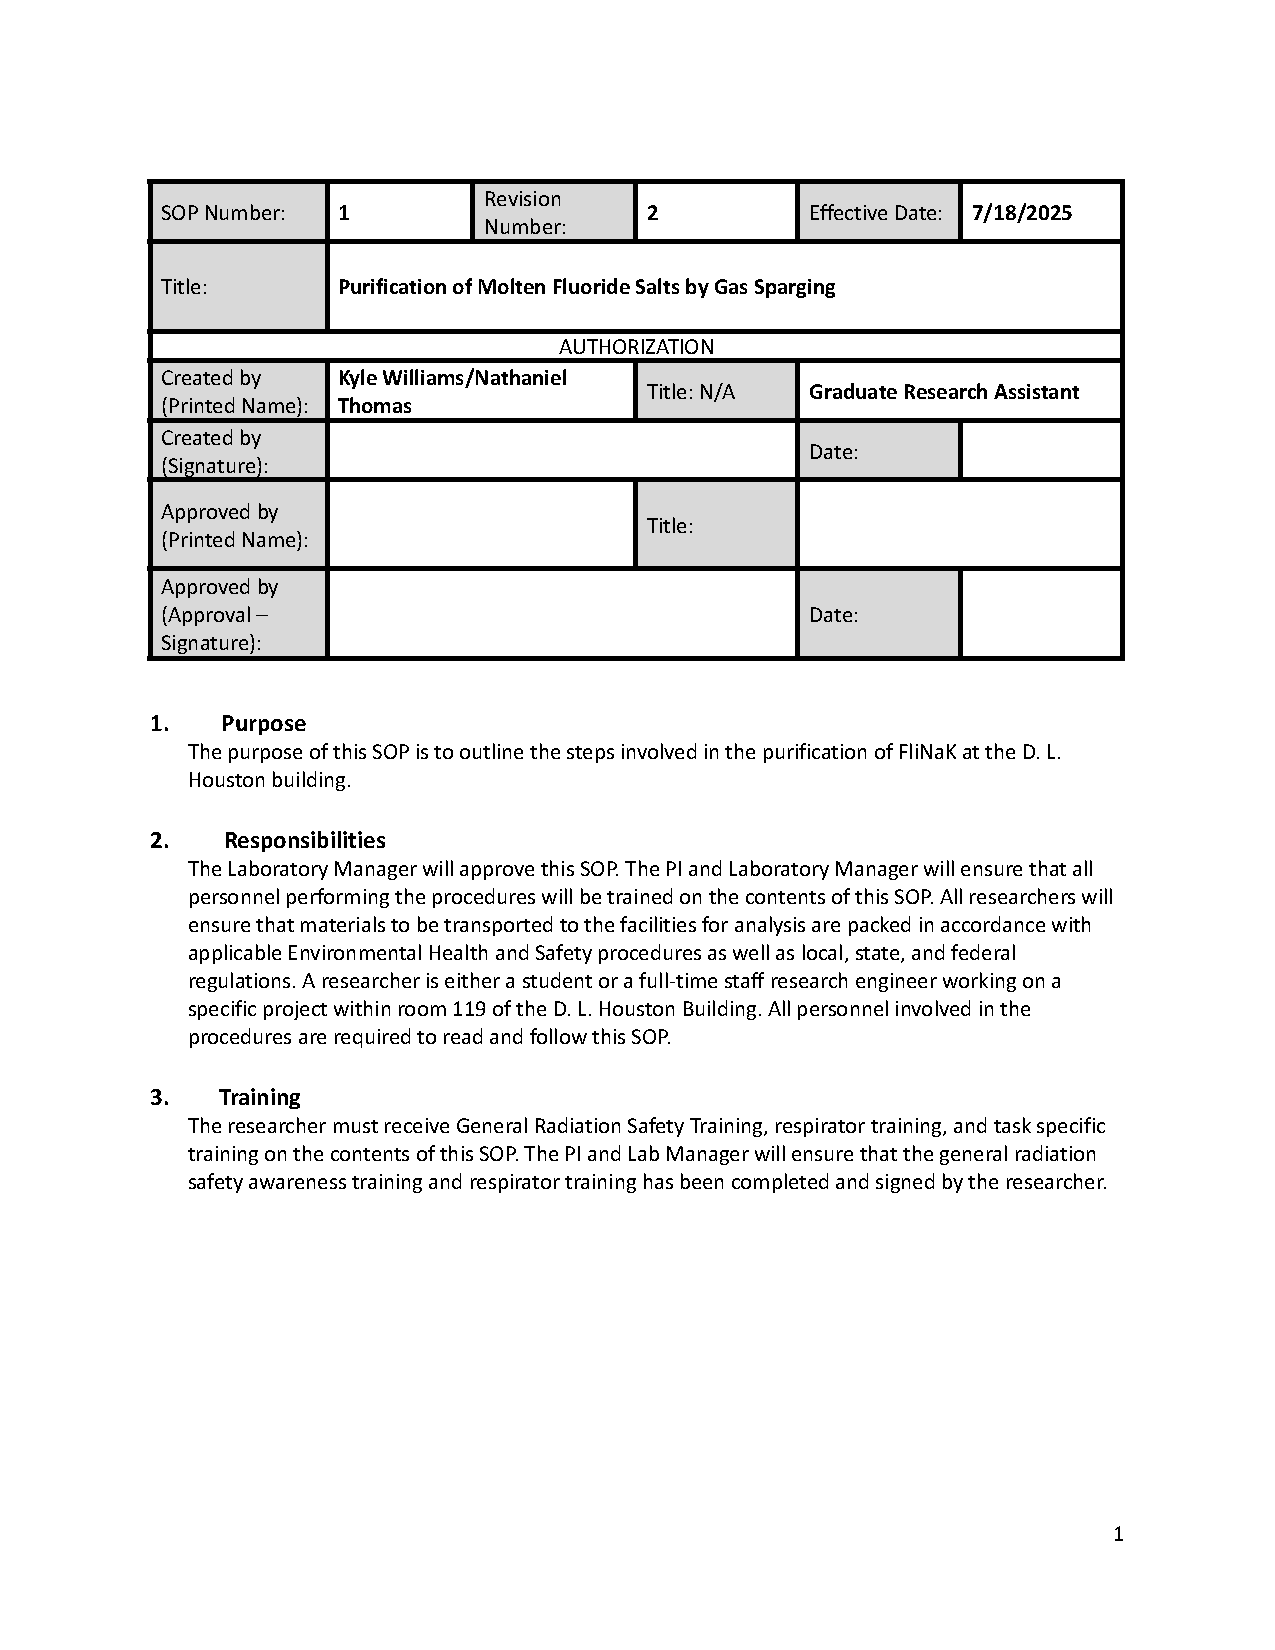
\includepdf[pages=-]{./assets/sop/sop.pdf}

This is the standard operating procedure for the FLiNaK purifier. The process
for running the purifier is broken into four distinct stages:

\begin{enumerate}
    \item \Cref{sec: loading}
  \item Drying and melting
  \item Purification
  \item Transfer
\end{enumerate}

\subsection{Loading}
\label{sec: loading}
The FLiNaK purifier is loaded through a 0.75" ID port on the top of the
purifier. This is shown in \Cref{fig:loading port}.

\begin{figure}[h]
  \centering
  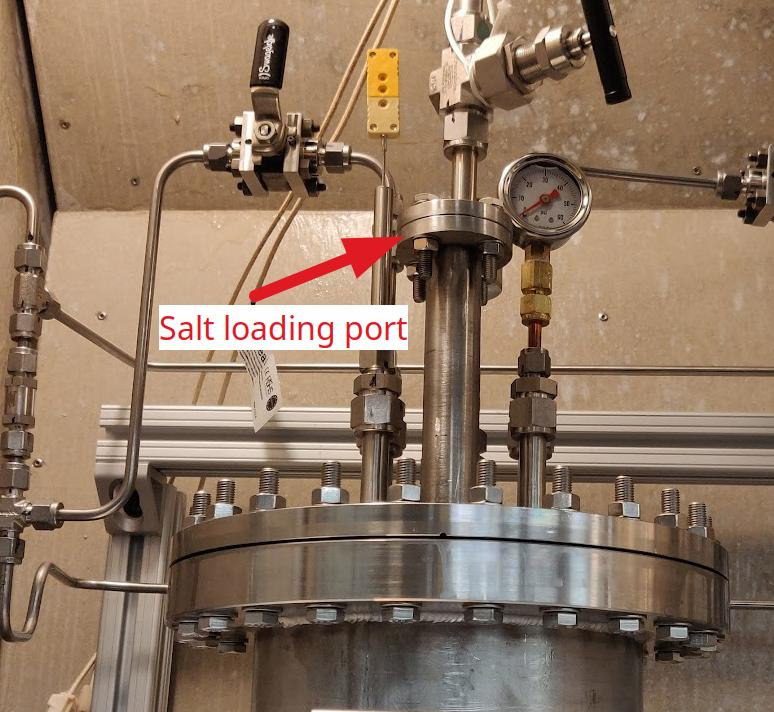
\includegraphics[width=0.4\textwidth]{./assets/pictures/loading port.jpg}
  \caption{The loading port for the reaction chamber.}
  \label{fig:loading port}
\end{figure}

% The following procedure assumes that as-recieved salt from Materion is
% being loaded into the purifier.

% \subsection{Scrubber preparation}

% Some consumables are used in the process of running the FLiNaK purifier.
% The following is required to prepare scrubbing for the system.

% \begin{enumerate}
%   \item \SI{200}{\gram} calcium hydroxide
%   \item \SI{2000}{\gram} potassium hydroxide
%   \item \SI{4}{gallons} of DI water
% \end{enumerate}

\pagebreak
